\documentclass{osa-article}

%% Select the journal you're submitting to
%% oe, boe, ome, osac, osajournal
\journal{osac}
% Key:
% Express journals must have the correct journal selected:
% {oe} Optics Express
% {boe} Biomedical Optics Express
% {ome} Optical Material Express
% {osac} OSAC Continuum
% Other OSA journals may use:
% {osajournal} Applied Optics, Advances in Optics and Photonics, Journal of the Optical Society of America A/B, Optics Letters, Optica, Photonics Research

% Uncomment if submitting to Photonics Research.
% ONLY APPLICABLE FOR \journal{osajournal}
% \setprjcopyright

% Set the article type
\articletype{Research Article}
% Note that article type is not required for Express journals (OE, BOE, OME and OSAC)

\usepackage{lineno}
\usepackage[clean]{svg}
\usepackage{subcaption}
\usepackage{mathtools}
\linenumbers

\begin{document}

\title{Time Domain Diffuse Raman Spectroscopy Using Single Pixel Detection}

\author{Alessandro Bossi,\authormark{1,*} Sanathana Konugolu Venkata Sekar,\authormark{2} Michele Lacerenza, \authormark{1} Stefan Sunsjar,  \authormark{2} Cosimo D’Andrea\authormark{1}, Renzo Vanna\authormark{1, 3}, Gianluca Valentini\authormark{1}, Andrea Farina\authormark{1}, Antonio Pifferi \authormark{1} }

\address{\authormark{1}Politecnico di Milano\\
\authormark{2}Sanatana\\
\authormark{3}CNR}

\email{\authormark{*}alessandro.bossi@polimi.it} %% email address is required

% \homepage{http:...} %% author's URL, if desired

%%%%%%%%%%%%%%%%%%% abstract %%%%%%%%%%%%%%%%
%% [use \begin{abstract*}...\end{abstract*} if exempt from copyright]

\begin{abstract}
\LaTeX{} manuscripts submitted to Optica Publishing Group journals may use these instructions and this universal template format. The template simplifies manuscript preparation and eases transfer between journals. \emph{Applied Optics}, JOSA A, JOSA B, \emph{Journal of Optical Communications and Networking}, and \emph{Photonics Research} authors should use the length-check template if a precise length estimate is needed. \emph{Optics Letters} authors and authors of short \emph{Optica} articles are encouraged to use the length-check template. Authors using this universal template will still need to adhere to article-length restrictions based on the final, published format.
\end{abstract}

%%%%%%%%%%%%%%%%%%%%%%%%%%  body  %%%%%%%%%%%%%%%%%%%%%%%%%%
\section{Introduction}
Raman spectroscopy provides information on the chemical composition of materials --- and in particular biological tissues --- with no need of labelling/staining and in principle non-invasively. Raman spectroscopy was typically limited to surface probing, as in microscopy. Recently, there was a strong impetus in extending Raman applicability to sub-surface probing of diffusive materials at depth of a few cm [SARA], opening the way to applications in several fields, from clinical diagnostics[REF] to cultural heritage[REF], from food assessment[REF] to quality control in pharma[Eliasson, C., & Matousek, P. (2007). Noninvasive authentication of pharmaceutical products through packaging using spatially offset Raman spectroscopy. Analytical Chemistry, 79(4), 1696-1701.], up to security controls at airports[REF].

Different approaches were proposed to study Raman signal in depths, such as Spatially Offset Raman Spectroscopy (SORS)[REF], Transmittance Raman Spectroscopy (TRS)[REF], Frequency Offset Raman Spectroscopy (FORS)[REF], Time-Domain Diffuse Raman Spectroscopy (TD-DIRS)[REF]. All of them share the same quest to cope the detection of Raman emission with photon random migration in highly diffuse media (e.g. biological tissues in the 600-1100 nm range), and can be grouped under the general field of Diffuse Raman Spectroscopy (DIRS). Each specific approach uses a different variable to yield a different depth sensitivity for Raman emitters. In particular, SORS exploits source-detector separation (larger distances leads to deeper penetration), FORS the excitation wavelength (different mean penetration depths depending on the spectral variation of the absorption and the scattering coefficient), TD-DIRS the photon arrival time (longer lived photons have travelled deeper into the medium). Conversely, TRS is not varying the depth selectivity based on an independent variable. Rather, the transmittance geometry --- whenever the probed medium permits --- provides an almost flat sensitivity for all Raman emitters located along the source-detector line, thus reducing the penalty loss of buried Raman signals. This geometry, implemented in multiple source-detectors pairs is also suitable for tomographic reconstruction, although signal paucity and sample/tissue accessibility is a great hurdle.

TD-DIRS is in principle very powerful since depth information is encoded in photon arrival time and no change in wavelength/collection is needed since photons can be classified based on their arrival time, while keeping the very same collection efficiency and collection geometry for all of them [REF]. Further, illumination/collection from the very same point in the Null Source-Detector Configuration is possible, with benefits in spatial resolution, signal intensity, probe handling[REF]. The key obstacles for TD-DIRS reside in the need for a short-pulsed (10-100 ps) yet narrowband (<1 nm) laser source and a parallel detector suitable to be coupled with a spectrometer and to measure photon arrival time at the single-photon level with ps temporal resolution. Indeed, the detector is the key limit factor since there is not the equivalent of a CCD (high quantum efficiency, high fill factor, high number of pixels) for time-domain single photon measurements. Initial attempts used intensified time-gated camera to suppress early photons by applying a programmable temporal gate window [REF]. Yet, these cameras are still too noisy to extract feeble Raman signals from biological tissues. An interesting perspective was opened by the availability of a time-correlated single-photon camera, yet the limited spectral range in the range >600 nm and the clipping to a max count rate of 1Mcounts/s were still an obstacle for \emph{in vivo} measurement. Arrays of Single Photons Avalanche Diodes (SPADs) are surely an interesting perspective for CMOS compatibility and on-chip integration with Time To Digital Converter (TDC) electronics. Yet, at present, the fill factor is still low, and first demonstration have been proposed for the rejection of fluorescence photons by time-gating but not for Diffuse Raman studies yet [REF].

The approach we propose in the present paper to overcome the limitations of current time-domain detectors is to adopt a compress sensing approach, where a single-pixel time-resolved detector is used in combination with a Digital Micromirror Device (DMD) which provides spectral sampling of the Raman signal. The signal dispersed through a standard spectrometer is filtered using the DMD with a 50\% ON/OFF pattern sequence and conveyed to the single-pixel detector. If a proper orthonormal basis is used sequentially (e.g. the Hadamard basis) and an inverse transform is applied, then the Raman spectra can be retrieved, preserving temporal information on photon arrival time.

The paper is organised as follows. First, we describe the experimental setup and provide basic performances (e.g. spectral resolution, temporal resolution). Then, Diffuse Raman spectra obtained from a two-layered tissue-equivalent phantom made of a scattering silicon slab on top of a marble (calcium carbonate) are shown, demonstrating increasing depth sensitivity for late arriving photons. Finally, the spectra of the upper and lower layer are retrieved using an inverse reconstruction algorithm based on a solution of the Diffusion Equation modified to describe diffuse Raman signals.


\section{Methods}
\subsection{System Setup}
Figure\ref{fig:complete_setup}(a) displays the scheme of the system setup, while Fig.\ref{fig:spectrometer}(b) highlights the layout of the the spectrometer, which follows the design proposed by\cite{Berto2017} to exploit a DMD for single-pixel measurements. As the illumination source, we used a custom tunable Ti:Sa laser with active mode-locking using acousto-optical modulation [REF]. The laser was pumped at 532 nm by the second harmonic of an Nd:Yag laser, yielding a train of pulses at a pulse repetition rate of 100 MHz, adjustable pulse width from 50 up to 500 ps, and tunable in the 680-880 nm range with a spectral width <0.1 nm [REF]. A small fraction of the laser beam was diverted to a detector by a beamsplitter to syncronise a Time-Correlated Single-Photon Counting Board (TCSPC) with the laser repetition rate.

Light injection and collection to/from the sample is arranged with a non-contact probe. On the excitation side, laser light is attenuated via a variable circular attenuator, coupled into a 1 mm core fiber, cleaned by a 10 nm bandpass filter at 780 nm to remove any unwanted spectral components, shaped using an axicon, and finally projected onto the sample to form a circular illumination. Changing the distance between the axicon and the focusing mirror permitted to vary the ring radius (from 000 mm up to 000 mm).

On the detection side, diffused light is collected from the center of the illuminated ring and coupled to a round-to-line optical fiber with seven cores of 200 $\mu m$ each with a numerical aperture of 0.2 by means of three lenses (L1,L2,L3) with a total magnification of 000. The object plane of the probe is placed 130 mm from the first lens. Inside the probe, elastically scattered light was removed by a 785 nm notch Filter with a band of 33 nm (XXX, Thorlabs).

In Time Domain Diffuse Raman, it is possible to measure at a fixed source detection separation $\rho$ as the depth separation of the Raman photons is encoded into time. It could be possible to measure at $\rho = 0$ to maximize the photon count. However, the diffuse optical approximations are not wholly verified, making the reconstruction of the measurements more challenging. Moreover, working at a higher $\rho$ reduces the intensity of the top layer and increases the photon ratio for the bottom layer photons. We opted for a source-detector separation of 6 mm.

The optical scheme of the spectrometer is presented in figure\ref{fig:spectrometer}. We used large 2 inches lenses to obtain a numerical aperture of 0.2 of the spectrometer and reduce the aberration. The 100 mm focal lenght lens L1 collimates light from the 100 $\mu m$ entrance slit onto the dispersion grating with 1200 lines/mm. The grating separates the light into the wavelength components. We selected the first mode of dispersion. A second 100 mm focal length lens L2 projects the image of the slit onto a DMD (DLP 6500, Texas Instruments) with a magnification factor of 1. The DMD is formed by a 1920 x 1080  micromirrors matrix that assumes two positions: +12° or -12°. The DMD has a size of 14 mm x 8 mm, with each mirror having a dimension of 7.6 $\mu m$. Using a homemade program, we can control the position of the mirrors. Photons reflected by the mirror at an angle of +12° are sent to the detector. Otherwise, they are removed. Thus, its is possible to filter the collected signal by a mask of \emph{0s} and \emph{1s} with any given pattern. The DMD dimension perpendicular to the wavelength dispersion was binned together to increase the photon count since it carries no spectral information. In principle, it could be used to attenuate the signal at wavelengths which could saturate the detector, but this is rarely the case with spontaneous Raman signals. The modulated light is sent to a pair of lenses (L3 focal distance of 100 mm, L4 focal distance of 50 mm) that focuses light with a magnification factor of 0.5 onto a single pixel hybrid detector (HPM100-50, Hamamatsu, Japan)[PICOQUANT?????] with dimensions of 6 mm x 6 mm. The detector had a spectral coverage from 400 nm to 900 nm (quantum efficiency: 000\% @ 000 nm and 000\% @ 000 nm), with a low dark countrate of 200 cps. A Time-Correlated Single-Photon Counting board (TCSPC) was used to process the flow of detected photons and generate the histogram of photon arrival times. The DMD sends a trigger signal to the TCSPC board every time the pattern changes to distinguish the measurement basis. Once the board receive the trigger, it starts a new recording.


\subsection{Retrieval of Raman spectra}
The set of patterns written on the DMD to filter the spectral signal can be decribed as a matrix \textbf{M}, where columns identifies the pattern on the DMD and rows host the ON/OFF sequence along the wavelength dimension. The array of measurements $\textbf{S}_{DMD}$ at the detector for a whole set of patterns can be expressed as a linear system of the real spectrum \textbf{S}_{wl}:

\begin{equation}
    \textbf{S}_{DMD} = \textbf{M} \textbf{S}_{wl}
    \label{eq:lin_DMD}
\end{equation}

The mode of operation of the spectrometer depends on the basis set that we upload to the DMD. There are two primary choices: Monochromator or Multiplex mode.
Using the Monochromator scan, the DMD shows a single line, and we collect a single wavelength at a time. In this case, in eq. \ref{eq:lin_DMD} $\textbf{M}$ is the identity matrix. An example of the pattern uploaded on the DMD is shown in fig. XXX. During a measurement, only 1/n times a line will be illuminated. Conversely, in the multiplex approach we send multiple wavelengths to the detector at a time. In particular we choose the Hadamard basis set. The DMD shows a Hadamard base at a time. In this case, in eq. \ref{eq:lin_DMD} $\textbf{M}$ is the Hadamard matrix. An example of the pattern uploaded on the DMD is shown in fig. XXX. We measure on the Hadamard basis set and then reconstruct the wavelength basis set during the data analysis. 
Solving the linear system we obtain $S_{wl}$
\begin{equation}
    \textbf{S}_{wl} = \textbf{H}^{-1} \textbf{S}_{DMD}
\end{equation}
Using the Hadamard scan each line is illuminated 50\% of the time.
This method can collect significantly more photons than the monochromator mode, reducing the tradeoff between resolution and time integration.

\subsection{Samples}
To study the depth propagation and verify the ability of our system for depth probing, we used a bilayer geometry composed on top of a silicone elastomer (PDMS) tailored to have $\mu_s = 10$ $cm^{-1}$ and $\mu_a = 0.10$ $cm^{-1}$  at 700 nm, with a thickness of 10 mm. We used a block of calcite with 2 cm thick 3cmx4cm on the bottom.
For the top layer, we chose a PDMS with the scattering coefficient of 10 $cm^{-1}$ because it simulates a biological tissue. We used calcite to simulate a bone.
We present in figure XXX the scattering and absorption coefficient for marble and the PDMS phantom measured using time-domain broadband diffuse optics. At 785 nm, the silicone layer has a scattering coefficient of 9 $cm^{-1}$ and calcite has a scattering coefficient of 12 $cm^{-1}$.


\begin{figure}
\begin{subfigure}{\textwidth}
    \centering
    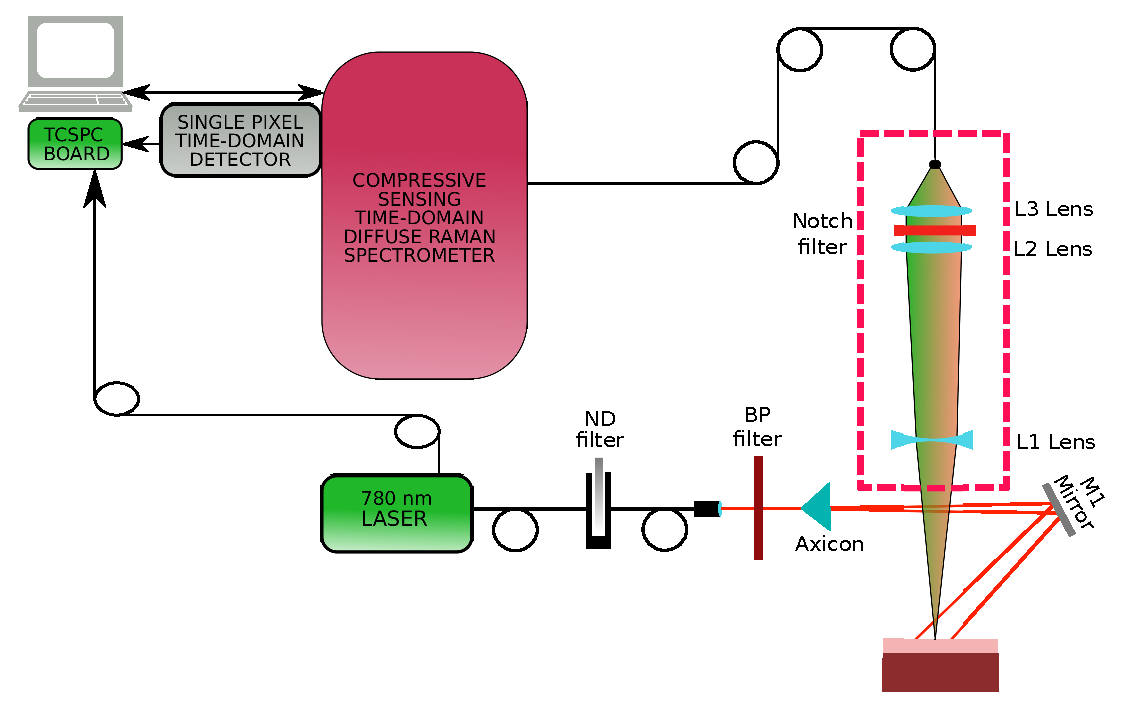
\includegraphics[scale = 0.5]{figure/schemesvg.eps}
    \caption{General scheme}
    \label{fig:complete_setup}
\end{subfigure}
\newline
\begin{subfigure}{\textwidth}
    \centering
    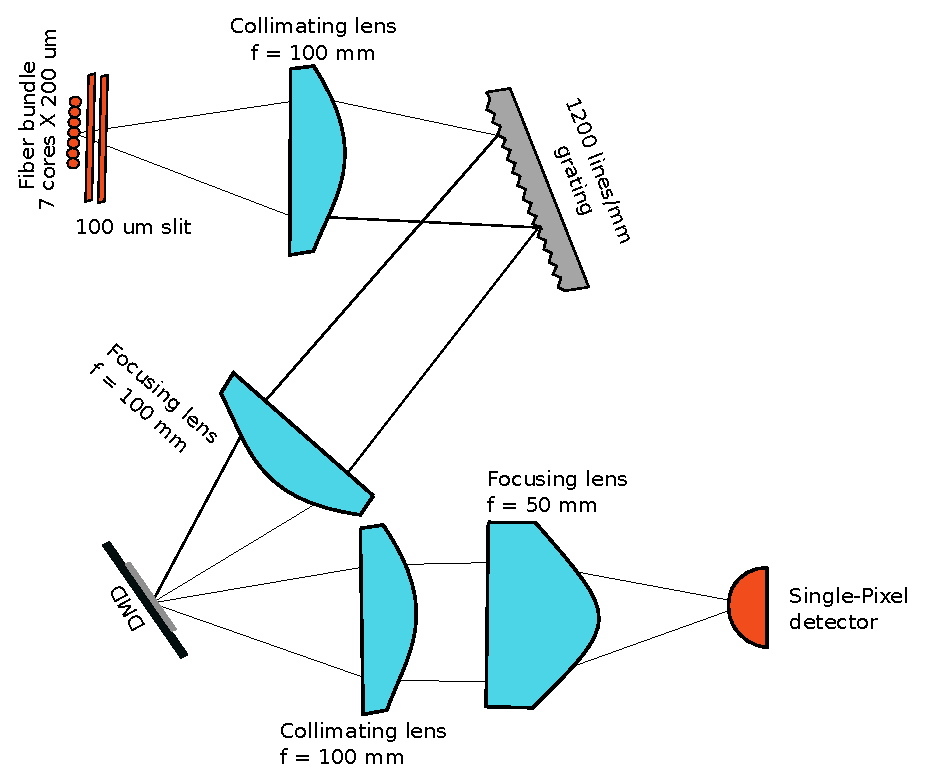
\includegraphics[scale = 0.5]{figure/spectrometer.eps}
    \caption{scheme of the spectrometer}
    \label{fig:spectrometer}
\end{subfigure}
\caption{schemes of the setup}
\label{fig:setup}
\end{figure}


\section{System Characterisation}
The spectrometer has a resolution of 0.8 nm or 11 $cm^{-1}$ at 850 nm as seen in figure \ref{fig:fwhm_spectra}.
To measure the resolution, we changed the wavelength of the laser to 852 nm that is included in the spectral range of the spectrometer. 
\begin{figure}
\begin{subfigure}{0.5\linewidth}
    \centering
    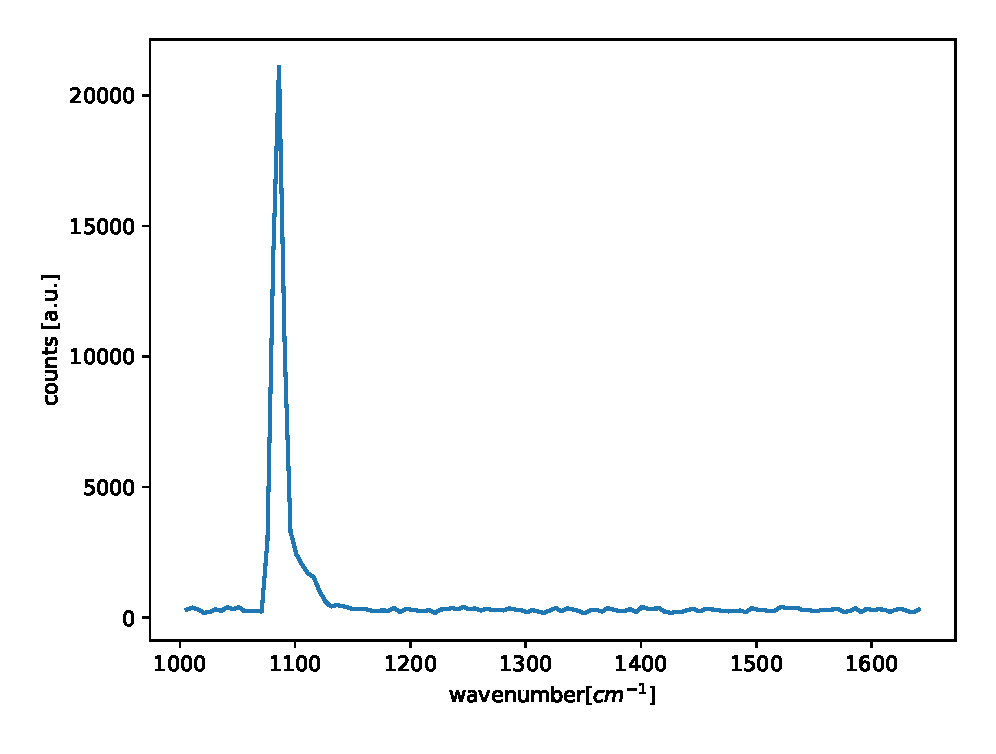
\includegraphics[scale = 0.4]{figure/fwhm_spectra.eps}
    \caption{Spectral resolution of the time-domain diffuse Raman spectrometer}
    \label{fig:fwhm_spectra}
\end{subfigure}
\begin{subfigure}{0.5\linewidth}
    \centering
    \includegraphics[scale = 0.4]{figure/time_domain_fwhm.eps}
    \caption{IRF of the system}
    \label{fig:td_fwhm}
\end{subfigure}
    \caption{Response of the system.}
\end{figure}

We illuminated a diffusive sample using the illumination scheme shown in \ref{fig:setup}. We do not connect the laser's output directly to the seven core fiber because we need to excite all the fiber cores and fiber modes as we have with Raman photons.
The spectral resolution depends on the image on the DMD plane and thus on the dimension of the input fiber parallel to the wavelength dispersion.
We added a slit aperture of 100 $\mu m$ to reduce the dimension of the image and improve the resolution at the cost of the optical efficiency.
The dimension of the slit currently limits the spectrometer's resolution.

The temporal resolution is measured by directly connecting the laser output to the seven core fiber. We excite all the fiber modes by adding a piece of Teflon at the connection of the 1 mm fiber to the seven core fiber.
We do not use a sample because we are interested in only the system's time response. The time of diffusion inside the Teflon with thickness of approximately 200 $\mu m$ is considered negligible compared to the system's response. We measured a temporal fwhm of 276 ps and is shown in figure \ref{fig:td_fwhm}. 

The elements that influence the temporal resolution of the system are the laser pulse, fiber broadening, broadening in the spectrometer and detector response.

We measured the optical efficiency of the spectrometer at 850 nm and found it to be 8\%. The photon loss of the spectrometer is caused by different modes of the grating, lenses, the fill factor of the DMD, and a slit aperture. The absolute efficiency of the spectrometer is approximately 2\% because the hybrid detector has 20\% efficiency at 850 nm.

The spectral range of the spectrometer is 50 nm or 700 $cm^{-1}$ at 850 nm.
The DMD can show up to 256 bases and therefore, we can collect up to 256 points.

We performed a first calibration of the spectrometer using a broadband source. 
Each measurement is fine-tuned using two reference peaks, one from silicone and one from calcite.


\section{Diffuse Raman Mesurements on Tissue Equivalent Phantoms}
To validate the system, we used a PDMS-Calcite phantom.
In figure \ref{fig:Marble_ref} we have the Raman spectra of calcite collected with our system. Calcite has an instense signal at 1085 $cm^{-1}$.

\begin{figure}
\begin{subfigure}{.5\textwidth}
    \centering
    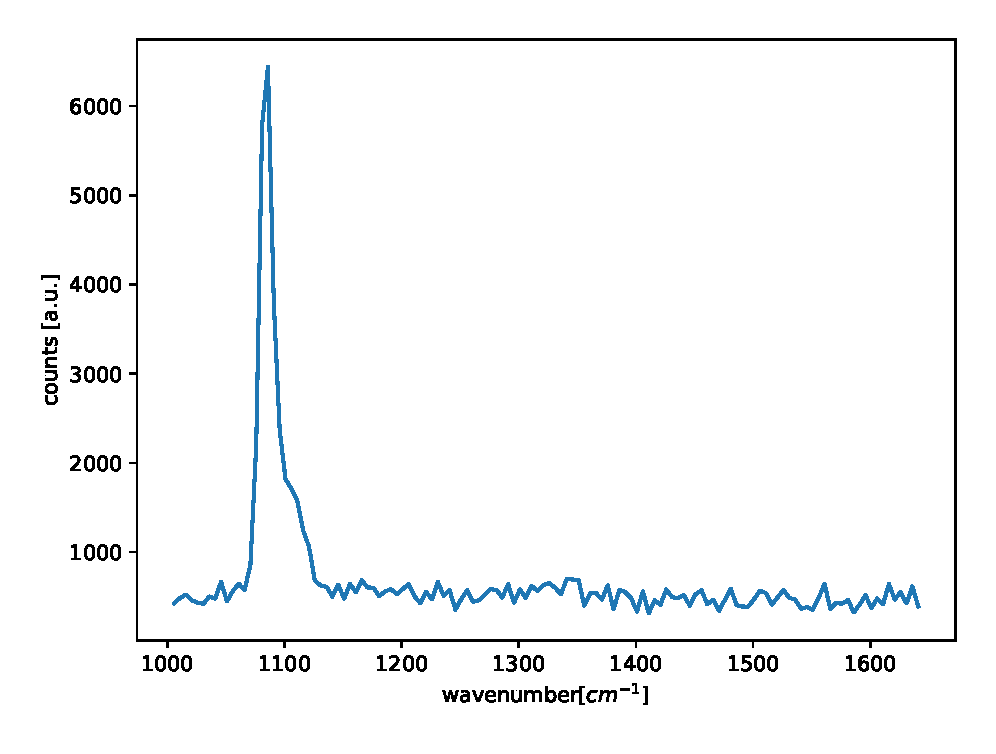
\includegraphics[scale = 0.4]{figure/spectra_marble.eps}
    \caption{Raman spectra of calcite measured with the current system}
    \label{fig:Marble_ref}
\end{subfigure}
\begin{subfigure}{.5\textwidth}
    \centering
    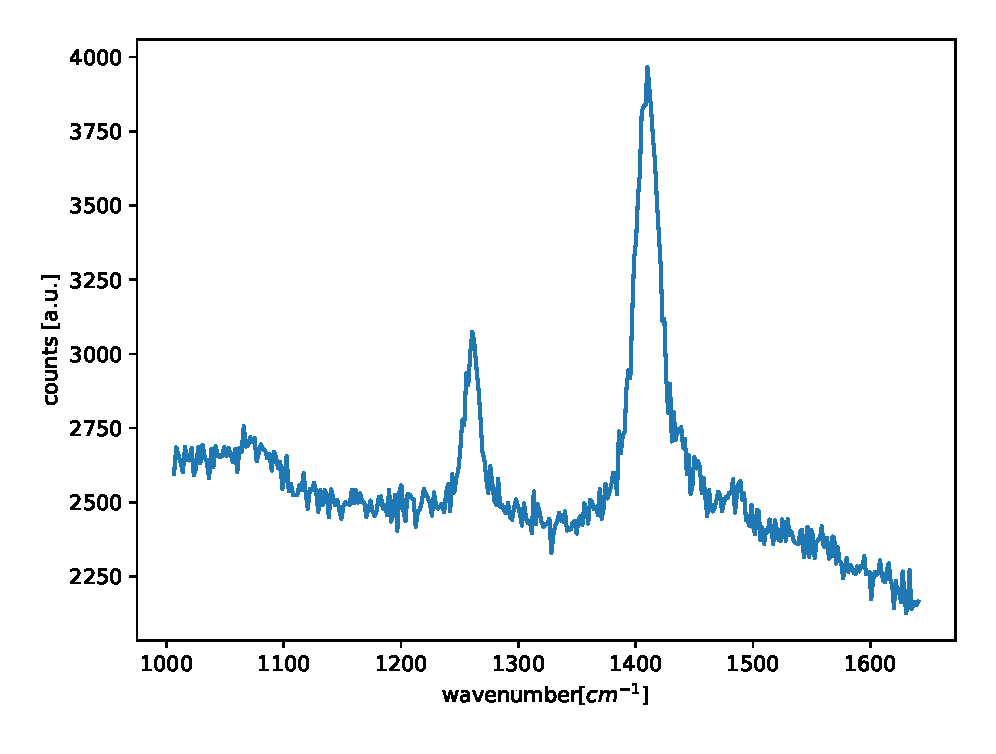
\includegraphics[scale = 0.4]{figure/spectra_PDMS.eps}
    \caption{Raman spectra of PDMS collected with Teledyne Princestone LS 785 spectrometer with Blaze camer}
    \label{fig:PDMS_ref}
\end{subfigure}
\caption{Reference spectra.}
\end{figure}
In figure \ref{fig:PDMS_ref} we have the Raman spectra of PDMS. It has a much weaker Raman intensity compared to calcite. Two Raman peaks are identifiable. One at 1411 $cm^{-1}$, the second at 1260 $cm^{-1}$.

\begin{table}
    \centering
    \begin{tabular}{|c|c|}
        \hline
        Foundamental spectra resolution & 11 $cm^{-1}$ \\\hline
        Temporal resolution & 276 ps \\\hline
        f-number & 2 \\\hline
        NA & 0.2 \\\hline
        slit-size & 100 $\mu m$ \\\hline
        number of points & 256 \\\hline
        optical efficiency & 10\% \\
        \hline
    \end{tabular}
    \caption{System specification}
    \label{tab:sys_spec}
\end{table}


\section{PHANTOM MEASUREMENTS}
We aim to demonstrate the ability of our system to differentiate the Raman photons from the top and bottom layers. 
Moreover, we aim to demonstrate a parallel approach, using the Hadamard matrix, to reduce the measurement integration time and noise over a monochromator approach in time domain and show the disentanglement of the temporal profile of the photons with different wavenumber.

The measurements were performed at 780 nm with 100 mW and 270 ps of fwhm and we collected using 128 bases with a source detection separation of 6 mm.
The integration time for every base is 6 s. The total integration time is  768 s ($\approx$ 12.5 minutes).

We performed the measurement using two modalities: Monochromator mode or Hadamard mode. The difference between these two modes is the basis set shown on the DMD.
The monochromator mode uses the trivial basis set where one line corresponds to a wavenumber. The Hadamard mode measures on a more complex set requiring the reconstruction onto the wavelength basis.

In figure \ref{fig:had_bi} and \ref{fig:mono_bi} we show the integration on time of the measurement performed using the two different modes with the same measurement time integration of 6 s per base. 
\begin{figure}
    \begin{subfigure}{0.5\linewidth}
        \centering
        \includegraphics[scale = 0.4]{figure/spectra_had.eps}
        \caption{Raman spectra of the bilayer phantom using Hadamard mode}
        \label{fig:had_bi}
    \end{subfigure}
    \begin{subfigure}{0.5\linewidth}
        \centering
        \includegraphics[scale = 0.4]{figure/spectra_mono.eps}
        \caption{Raman spectra of the bilayer phantom using the monochromator mode}
        \label{fig:mono_bi}
    \end{subfigure}
    \caption{Raman spectra measured with the two modalities.}
\end{figure}

The Hadamard mode's main advantage is that we can collect significantly more photons than the monochromator mode. In fact, the Hadamard measurement has significantly less noise compared to the Monochromator. In the Monochromator mode, we collected 43495 photons. In the Hadamard mode, we collected 1165311 photons. We collect 22 times more photons. Considering the Poisson noise it improves the signal-to-noise ratio by a factor $\sqrt{n}$ the signal-to-noise ratio is 4.7 times the one with the monochromator mode. We are particularly sensitive to noise because we require a significant photon count at every time gate.

From the continuous wave measurement in figure \ref{fig:had_bi} we can recognize three strong peaks one at 1086 $cm^{-1}$, 1411 $cm^{-1}$, and a smaller one at 1260 $cm^{-1}$.
However, it is impossible to distinguish the depth origin of the Raman peaks. For this, we have to look also at the time of arrival of the photons.
The complete measurement is presented in a 2D plot in figure \ref{fig:2D} where the wavenumber is presented on the y-axis, on the x-axis is presented the time in ps and the photon count at each time-gate of a single wavenumber is codified by the color. 
In some time-gates, we report a negative photon count. This is an artifact introduced by the Hadamard reconstruction.
In figure \ref{fig:2D} three strong signals are again recognizable. We observe that the stripe at $1086 cm^{-1}$ wavenumber is delayed compared to the other two. This signal comes from the Raman photons of the marble at depth.  
\begin{figure}
    \centering
    \includegraphics[scale = 0.4]{figure/2D.pdf}
    \caption{Two-dimensional representation of the measurement.}
    \label{fig:2D}
\end{figure}
To better visualize the time delay and appreciate the depth probing capabilities of time in figure \ref{fig:multi_time} we bin the measurement in 8 gates and plot the spectra at each time gate. In the first gate we show photons that arrive at a time lower than 270 ps and we can measure only Raman photons with 1411 $cm^{-1}$ and 1260 $cm^{-1}$. Those photons are the Raman signature of PDMS and they come from the top layer. In the second time-gate, we observe the slow rise of the signal at 1086 $cm^{-1}$. It is the Raman signature of calcite of the bottom layer. In the fourth gate, it is possible to observe the maximum intensity of the calcite peak and see that the Silicon photons are nearly extinguished. In the following gates, the Raman signal of the calcite also slowly decreases.
We can see that the signals coming from the two-layer have different temporal evolution. To better appreciate it we have to show the time profile of the Raman photons of the different layers.
The temporal profile for the Raman signals is obtained by integrating over the spectral fwhm. The temporal profile shown in figure \ref{fig:Raman_tProfile}  for the bottom layer was taken at 1086 $cm^{-1}$ and at 1411 $cm^{-1}$ it was taken for the top layer. The peak intensity of the top layer shown in figure  \ref{fig:multi_time} is greater than the one from the bottom layer in figure \ref{fig:Raman_tProfile}. This is due to the larger photons spread in wavenumber in silicone. 

\begin{figure}
    \centering
    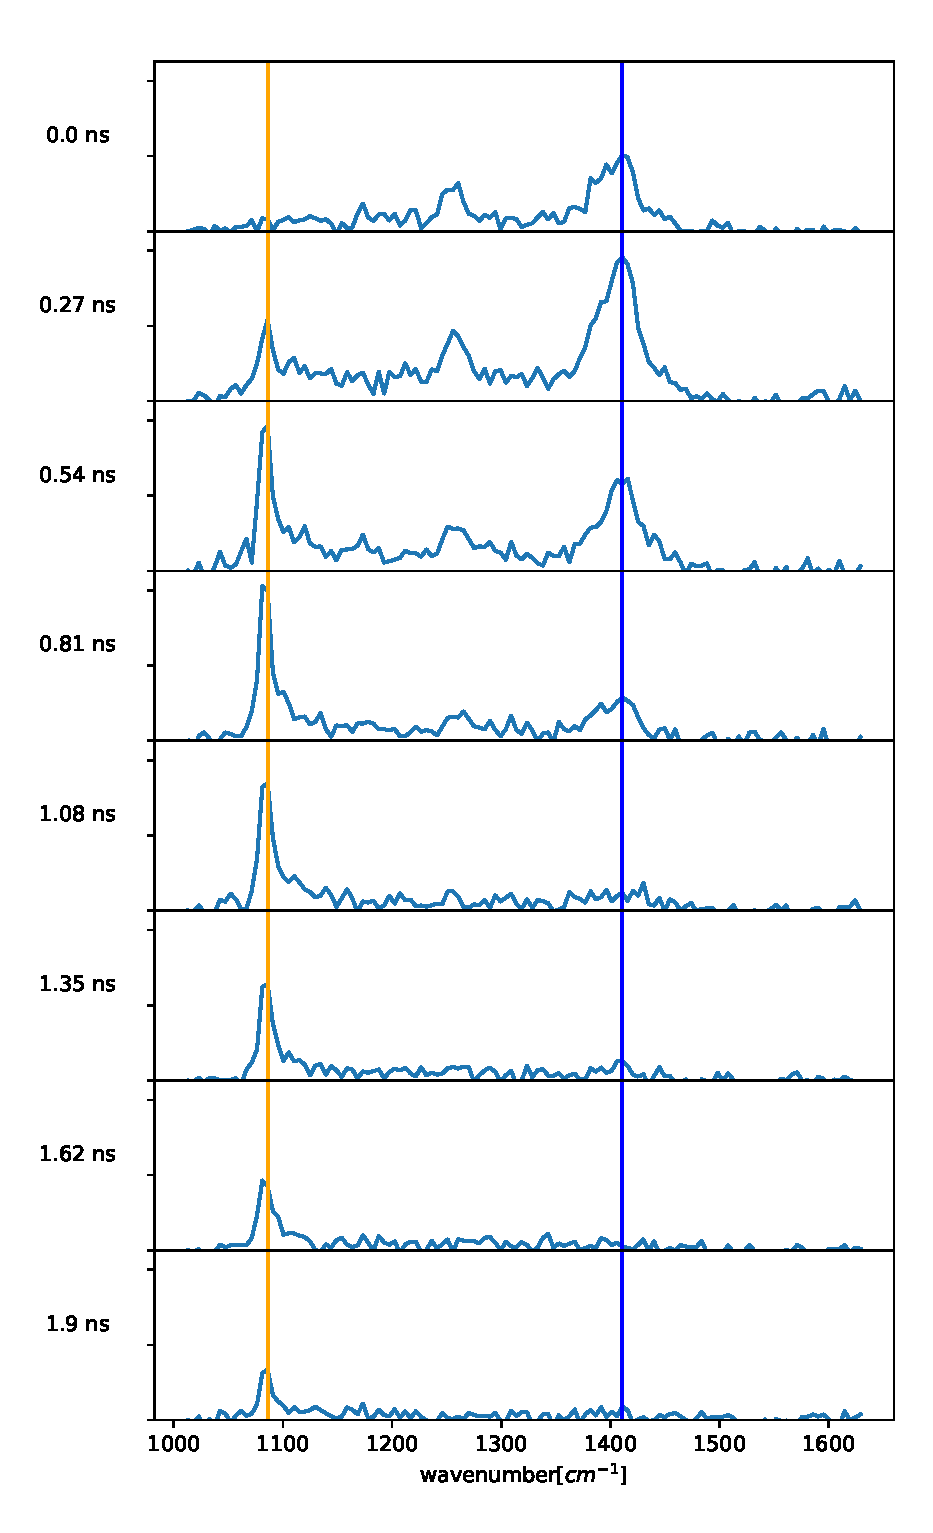
\includegraphics[scale = 0.4]{figure/multi8_time.eps}
    \caption{Binning of the photons}
    \label{fig:multi_time}
\end{figure}

As highlighted previously, the photons from the bottom layer arrive later than those from the top. It is due to the added travel path of photons inside the first layer required to reach the calcite. In fact, due to the longer travel path, the response to the impulse of the bottom layer is longer than the one from the top. As a result, the Raman photons from the bottom layer have a slower response time than the ones from the top.

In figure \ref{fig:enh} we present the enhancement factor calculated following the method presented in \cite{Sekar2017}:
\begin{equation}
\eta= \frac{\frac{I_{bottom}(t)}{I_{top}(t)}}{\frac{I_{bottom}(t_0)}{I_{top}(t_0)}} 
\label{eq:enh}
\end{equation}
\begin{figure}
\begin{subfigure}{0.5\linewidth}
    \centering
    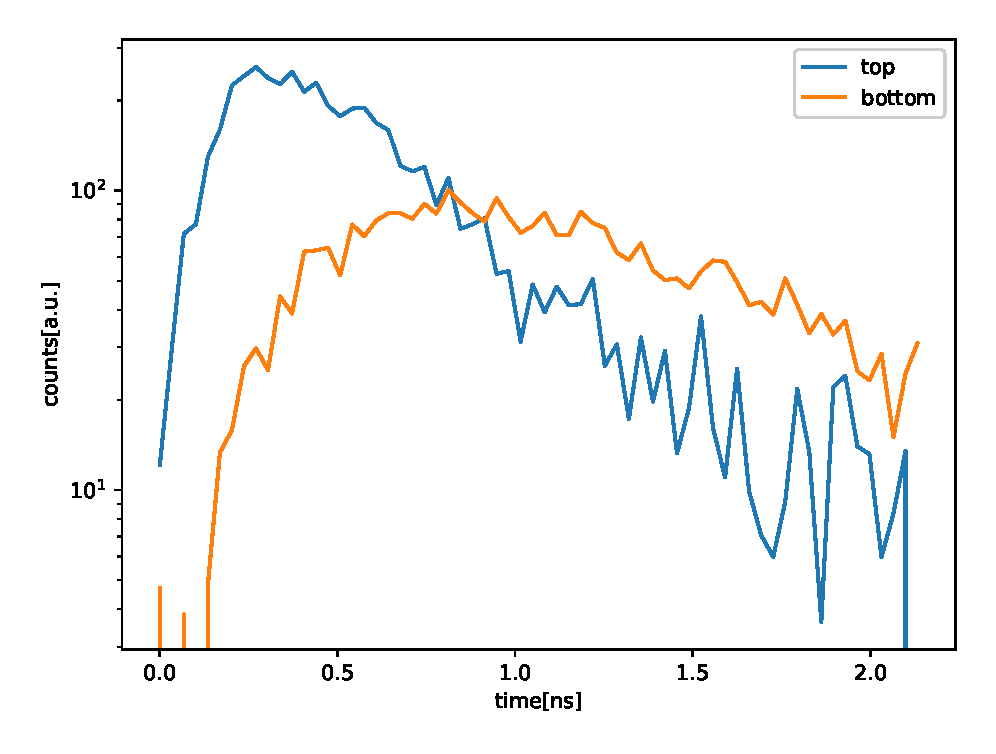
\includegraphics[scale = 0.4]{figure/top_bottom_time.eps}
    \caption{Temporal profile of the top's and bottom's layer photons}
    \label{fig:Raman_tProfile}
\end{subfigure}
\begin{subfigure}{0.5\linewidth}
    \centering
    \includegraphics[scale = 0.4]{figure/enh.eps}
    \caption{Enhancement factor calcuolated using \ref{eq:enh}}
    \label{fig:enh}
\end{subfigure}
    \caption{Temporal evoluition of the Raman signal}
\end{figure}
The enhancement factor is the bottom/top ratio over a constat to normalize over the Raman intensity.
The photons from the bottom layer in the later gates reach an enhancement factor of 70. However, after 1500 ps there are numerical issues because there are too few photon counts from the top layer, so it is no longer possible to use the enhancement factor.
To improve the enhancement we could increase the source detection distance at the cost of photons collected.



\section{Two-Layer Reconstruction}
In the previous section, we presented the results of our experiments and highlighted the relationship between time and depth. However, we want also to reconstruct the Raman scattering coefficient of each layer separately.
The forward model of the Raman scattering in diffusive media is based on \cite{Martelli2016} where a heuristic approach for the Raman propagation in a diffusive medium is presented. In a bilayer geometry, given the thickness of the two materials and optical parameters, we can find the response to the impulse of Raman photons from the top layer ($W_{top\tilde{\omega}}$) and from the bottom ($W_{bottom\tilde{\omega}}$).
The forward model is equal to 
\begin{equation}
\textbf{I} = [W_{top}  W_{bottom}] \begin{bmatrix}
                                \mu_{R,top}\\
                                \mu_{R,bottom}
                            \end{bmatrix}
\end{equation}
where I is the ideal response of the system and $\mu_{R,top}$, $\mu_{R,bottom}$ are the Raman scattering coefficients for the top and bottom layers.

We also need to consider the spectrometer's impulse response in the real case. We find the real signal by convolving the impulse response to the impulse response of the sample:
\begin{equation}
M = IRF * \textbf{I}
\end{equation}
 The spectrometer has been designed to remove the probing light. Therefore, we cannot directly measure the IRF of the system. We can extrapolate the IRF using one Raman peak. We know that:
\begin{equation}
M_i =  \bar{\mu_{R,i}} IRF * W_i 
\label{eq:find_irf}
\end{equation}
We use the signal of the top layer (PDMS) presented in figure \ref{fig:Raman_tProfile}. This approach is justifiable if we assume that the top layer is easily accessible for chemical inspection and its Raman signal can be known.
Deconvolving equation \ref{eq:find_irf} we obtain the IRF.
We can solve the linear system presented in eq. \ref{eq:find_irf}.
In figure \ref{fig:reconstruction} we present the reconstruction of the measurement performed with the Hadamard mode presented in the previous section.
We observe the separation of the scattering coefficient of the bottom layer from the one from the top.
\begin{figure}
    \centering
    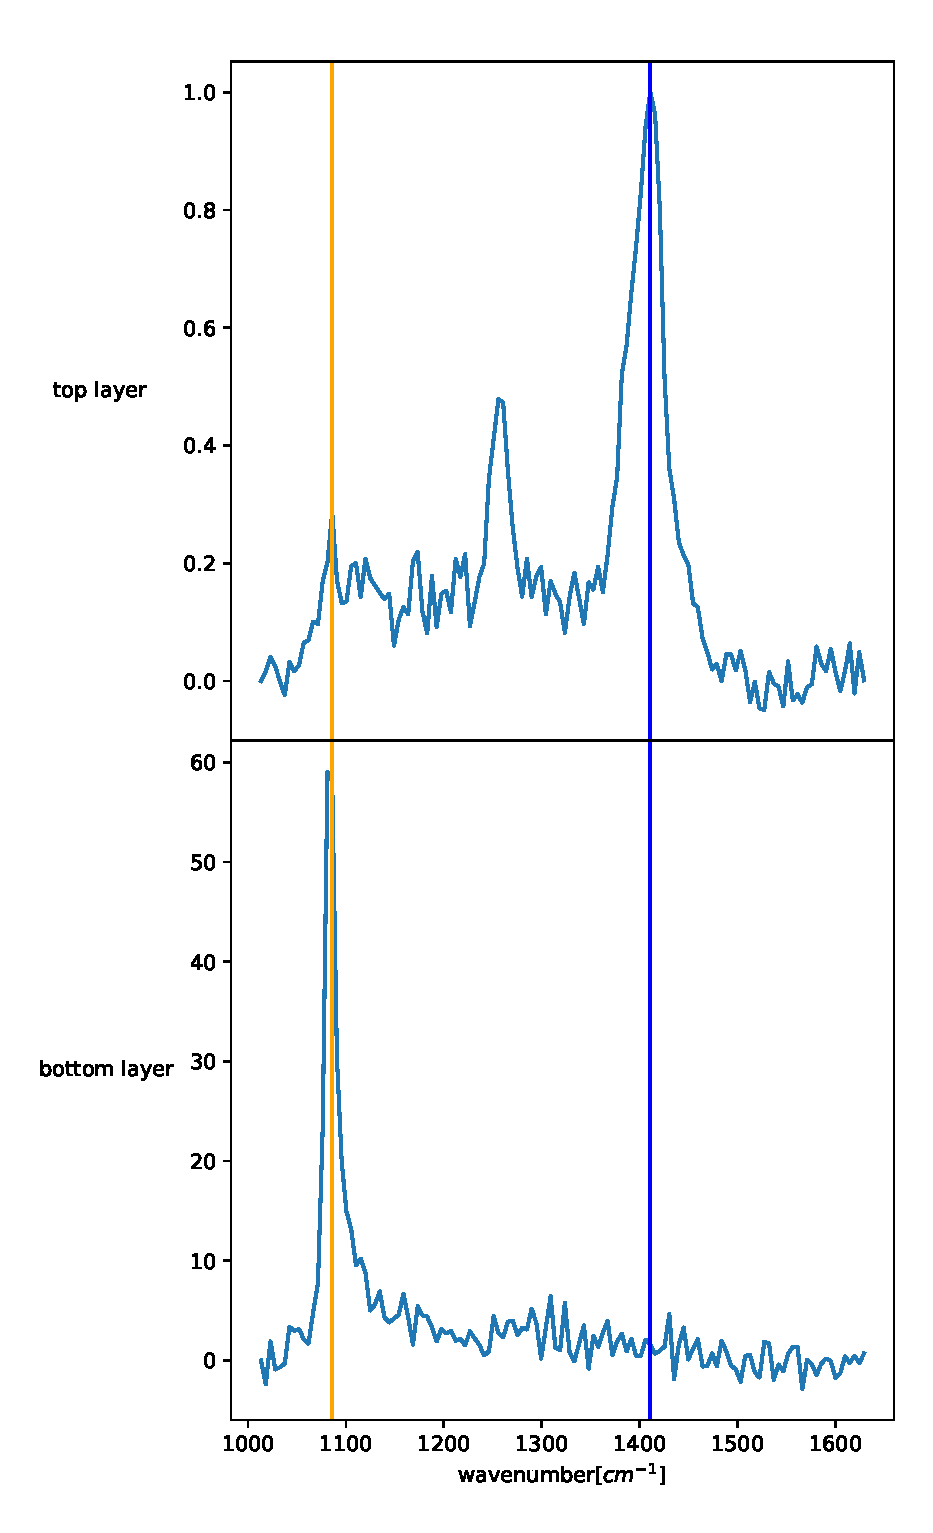
\includegraphics[scale = 0.4]{figure/recons.eps}
    \caption{Two layer Raman scattering coefficient reconstruction. Intensity normalized with the maximum of the top layer.}
    \label{fig:reconstruction}
\end{figure}
In the top layer reconstruction, we notice a small peak at 1086 $cm^{-1}$ in correspondence to the Raman peak of calcite of the bottom layer. This is caused by the uncertainty in the measurement of the IRF, uncertainties in the measurements of the optical parameters or issues with the model caused by the diffuse optical approximation.


Following the approach of \cite{depthLight} using the previous model we performed a coarse calibration of time to depth position.
We present in figure \ref{fig:time_depth} the function of maximum depth with time.
\begin{figure}
    \centering
    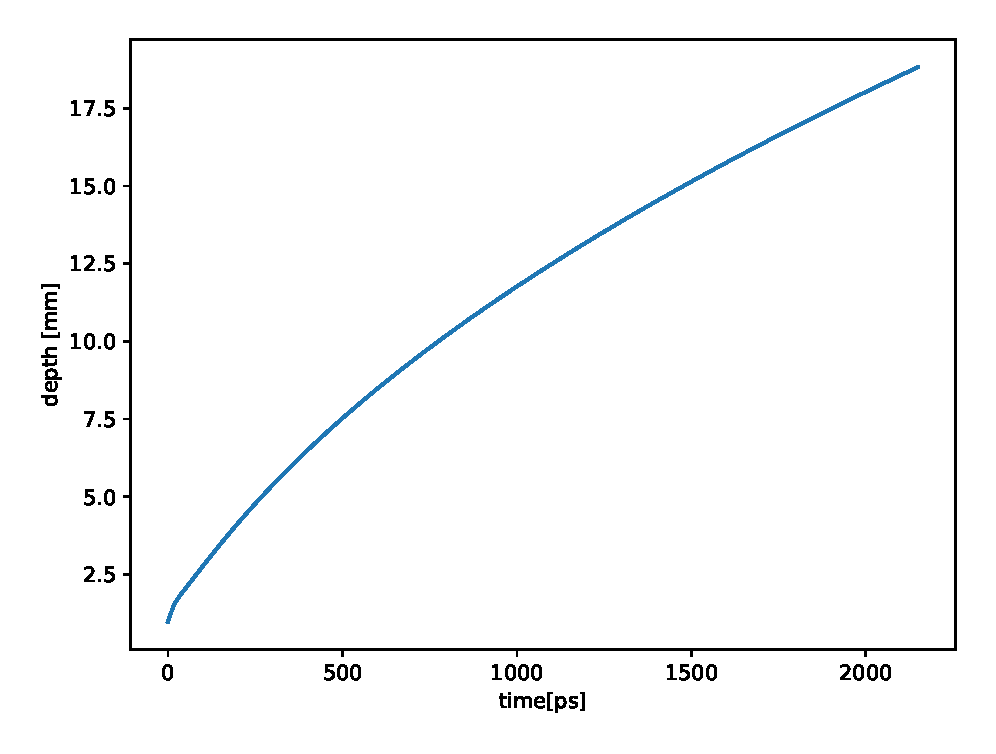
\includegraphics[scale = 0.4]{figure/time_depth_conv.eps}
    \caption{Time to depth calibrtation}
    \label{fig:time_depth}
\end{figure}
Using this function we can convert the time into the depth position of figure \ref{fig:multi_time} in figure \ref{fig:spectra_depth}.
\begin{figure}
    \centering
    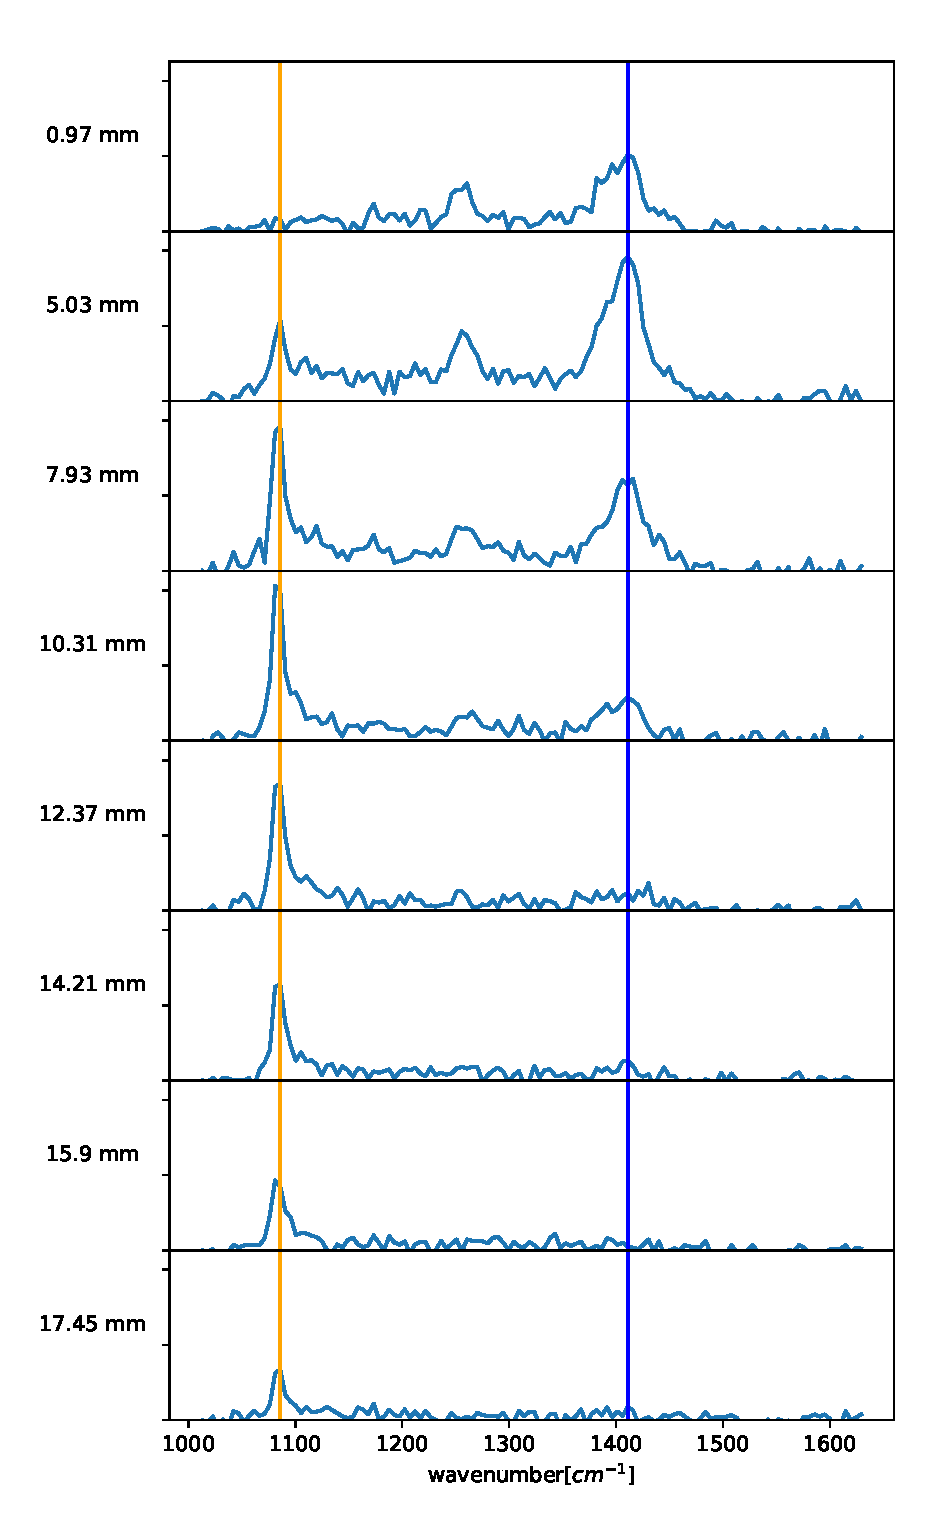
\includegraphics[scale = 0.4]{figure/multi8_depth.eps}
    \caption{spectra at depth}
    \label{fig:spectra_depth}
\end{figure}
\section{Conclusion}
After proofreading the manuscript, compress your .tex manuscript file and all figures (which should be in EPS or PDF format) in a ZIP, TAR or TAR-GZIP package. All files must be referenced at the root level (e.g., file \texttt{figure-1.eps}, not \texttt{/myfigs/figure-1.eps}). If there are supplementary materials, the associated files should not be included in your manuscript archive but be uploaded separately through the Prism interface.

%%%%%%%%%%%%%%%%%%%%%%% References %%%%%%%%%%%%%%%%%%%%%%%%%

Add references with BibTeX or manually.
\cite{Zhang:14,OSA,FORSTER2007,Dean2006,testthesis,Yelin:03,Masajada:13,codeexample}

%%%%%%%%%% If using BibTeX:
\bibliography{article}

%\begin{figure}[htbp]
%\centering\includegraphics[width=7cm]{osafig1}
%\caption{Sample caption (Fig. 2, \cite{Yelin:03}).}
%\end{figure}

\end{document}
